% Chapter 1
%\newcommand {\DF}[2]{{\displaystyle\frac{#1}{#2}}}
\chapter{Tunnelling Spectroscopy with Proximity Effect} % Write in your own chapter title
\label{Chapter3}
\lhead{Chapter 3. \emph{Tunnelling Spectroscopy with Proximity Effect}} % Write in your own chapter title to set the page header

Our group currently have a featured paper published containing the topic of proximity effect in $d$-wave. It is interesting to propose a theory calculating the $d$-wave conductance accounting for the proximity effect. The work is in progress.
\section{Bogoliubov Equations}
As a matter of fact, the tunnelling conductance discussed in the previous chapter is based on a specific case which is shown in Fig.2.2, where the potential is assumed as a $\delta$ function and the pair potential is assumed as a step function, so that Bogoliubov  equations(3.1) have an analytical solution, which in contrast, no longer exists when dealing with more complicated case, such as accounting for proximity effect.
\subsection{Simplification for Bogoliubov Equations}
The general Bogoliubov equations are 
\begin{eqnarray}
i\hbar\frac{\partial f}{\partial t} = \Big(-\frac{\hbar^2}{2m}\frac{\partial^2}{\partial {x^2}}-\mu(x)+V(x)\Big)f(x,t)+\Delta(x)g(x,t)\nonumber\\
\\
i\hbar\frac{\partial g}{\partial t} = \Big(-\frac{\hbar^2}{2m}\frac{\partial^2}{\partial {x^2}}-\mu(x)+V(x)\Big)g(x,t)+\Delta(x)f(x,t)\nonumber
\end{eqnarray}
(3.1) has the solution form 
\begin{eqnarray}
\varphi(x,t)=
\left(\begin{array}{c}
f(x,t)\\
g(x,t)
\end{array}\right)
\end{eqnarray}
where $\mu(x),\Delta(x),V(x)$ are chemical potential, energy gap, and the ordinary potential which is related to barrier hight, in which we are interested in the latter two.
By introducing a solution of the form
\begin{eqnarray}
f=u(x)e^{ik_Fx-\frac{iEt}{\hbar}}\nonumber\\
\\
g=v(x)e^{ik_Fx-\frac{iEt}{\hbar}}\nonumber\
\end{eqnarray}
The Bogoliubov equations could be written in this way neglecting higher order terms\citep{Reference4}.
\begin{eqnarray}
&&\DF{\partial u}{\partial x}=i(\pi \xi_0\Delta_{\infty})^{-1}[Eu-\Delta(x)v]\nonumber\\
&&\\
&&\DF{\partial v}{\partial x}=-i(\pi \xi_0\Delta_{\infty})^{-1}[Ev-\Delta(x)u]\nonumber
\end{eqnarray}
which are the equations we are interested in, $\xi_0$ is the coherence length.

\subsection{A Mathematical Approach to Solve the Equation}
Various authors have conducted research on solving the Bogoliubov equations\cite{Reference6,Reference4}. Here we propose a numerical approach method though not implemented to solve the equations. Let the equations (2.4) have the solution form
\begin{eqnarray}
\phi(x)=
\left(\begin{array}{c}
u(x)\\
v(x)
\end{array}\right)
\end{eqnarray}
BdG equations could written in a matrix way,
\begin{eqnarray}
\left(
\begin{array}{cc}
 \frac{d}{dz}& 0\\
 0& \frac{d}{dz}  \\
 
\end{array}
\right)\phi=
\left(
\begin{array}{cc}
 \beta E& 0\\
 0& \beta E  \\
 
\end{array}
\right)\phi+
\left(
\begin{array}{cc}
 0& -\beta \Delta\\
  \beta \Delta& 0  \\
 
\end{array}
\right)\phi
\end{eqnarray}
in other words,
\begin{eqnarray}
D\phi=(I+M)\phi
\end{eqnarray}

We define an newly introduced solution to the following differential equations,
\begin{eqnarray}
D\phi_0=I\phi_0
\end{eqnarray}
which can be easily solved,
\begin{eqnarray}
\phi_0=
\left(
\begin{array}{c}
 e^{\beta E z}\\
 e^{-\beta E z}  \\
 
\end{array}\right)
\end{eqnarray}

We set that the final solution by introducing a new matrix,
which can be easily solved,
\begin{eqnarray}
\phi= P\phi_0=
\left(
\begin{array}{cc}
 p_1&0\\
 0&p_2  \\
 
\end{array}\right)\phi_0
\end{eqnarray}

We could derive that,
\begin{eqnarray}
D(P\phi_0)=(I+M)(P\phi_0)
\end{eqnarray}
and that,
\begin{eqnarray}
(DP)\phi_0=(MP)\phi_0
\end{eqnarray}

Therefore, if we focus on the matrix P, we could reason that,
\begin{eqnarray}
\frac{d}{dz}P=TP
\end{eqnarray}
or 
\begin{eqnarray}
\frac{d}{dz}P=
\left(
\begin{array}{cc}
 0& -\beta\Delta e^{-2\beta E x}\\
 \beta\Delta e^{2\beta E x}&0  \\
 
\end{array}\right) P
\end{eqnarray}

An approximated way is to compare to the interaction picture,
\begin{eqnarray}
P=\int TP_0 dz+\int T' dz'\int P'TP_0 dz+\cdots
\end{eqnarray}

This method is mathematically clear but computationally confusing. Therefore we didn't implement this method as we have another clear way discussed by the reference\citep{Reference4}

\subsection{Solving the Bogoliubov Equations}
We divide the tunnelling axis into four regions, named 'super','reduced','induced','normal', respectively, which is shown in Fig.3.1, where we already choose parabolic shape for the pair potential.
\begin{figure}[htbp]
\small
	\centering
		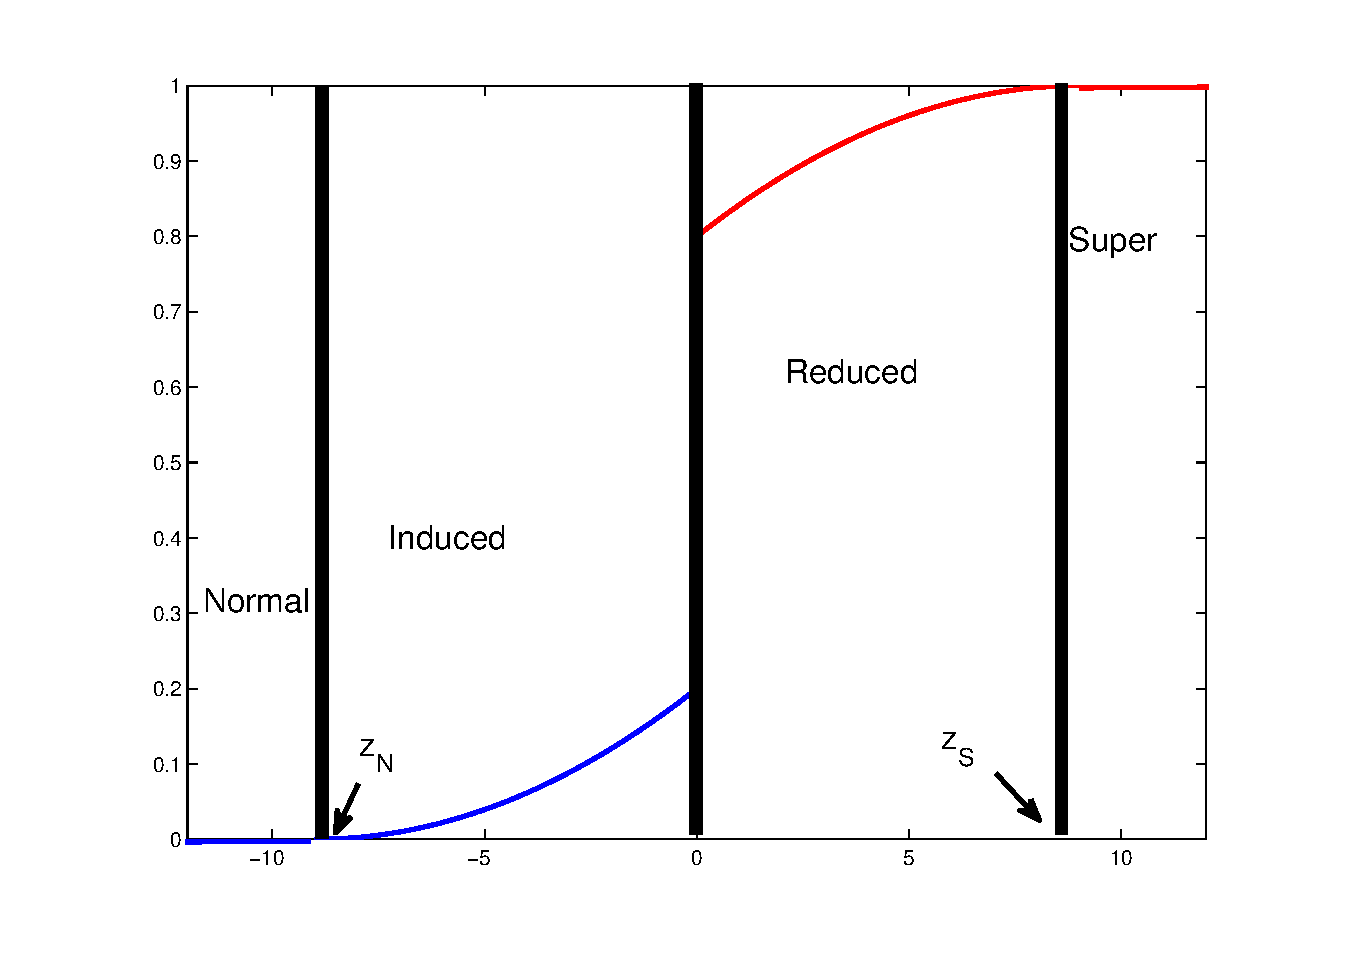
\includegraphics[width=10cm]{./Figures/3-2-1.eps}
		\rule{35em}{0.5pt}
	\caption[An Electron]{Parabolic shapes of reduced and induced pair potential. The tunnelling axis is divided into four regions.}
	\label{fig:Electron}
\end{figure}
In the 'super' region, the solution has the form of (3.16).
\begin{eqnarray}
&&\varphi_1=
\left(
\begin{array}{c}
 u_0\\
 v_0
 \end{array}\right)e^{i(k_F+k_S)x}\nonumber\\
&&\\
&&\varphi_2=
\left(
\begin{array}{c}
 v_0\\
 u_0
 \end{array}\right)e^{-i(k_F-k_S)x}\nonumber
\end{eqnarray}
where parameters are already known,
\begin{eqnarray}
u_0^2=1-v_0^2=\frac{1}{2}\Big(1+\frac{(E^2-\Delta_{\infty}^2)^{\frac{1}{2}}}{E}\Big)
\end{eqnarray}
and 
\begin{eqnarray}
k_S=(E^2-\Delta_{\infty}^2)^{1/2}(\pi \xi_0 \Delta_{\infty})^{-1}
\end{eqnarray}
The solution of this region serves as the generator of boundary conditions for the solution of the next region,'super'.
\begin{eqnarray}
&&u_{a1}(x_S)=u_{b2}(x_S)=u_0 e^{ik_Sx_S}\nonumber\\
&&v_{a1}(x_S)=v_{b2}(x_S)=v_0 e^{ik_Sx_S}\nonumber\\
&&\\
&&u_{b1}(x_S)=u_{a2}(x_S)=0\nonumber\\
&&u_{b1}(x_S)=u_{a2}(x_S)=0\nonumber
\end{eqnarray}
which is for the solution form of the region 'reduced', in which term $x_S$ is described in Fig.3.1, so does term $x_N$. The solution of reduced region is like (3.20).
\begin{eqnarray}
\varphi_j=
\left(
\begin{array}{c}
 u_{aj}\\
 v_{aj}
 \end{array}\right)e^{ik_Fx}+
 \left(
\begin{array}{c}
 u_{bj}\\
 v_{bj}
 \end{array}\right)e^{-i k_Fx},j=1,2
\end{eqnarray}

After obtaining the numerical solutions for (3.20), we select the values of only one point, which is at $x=0$
\begin{eqnarray}
&&u_{a1}(0)=u_{b2}(0)=u_{a1}^+\nonumber\\
\\
&&v_{a1}(0)=v_{b2}(0)=v_{a1}^+\nonumber
\end{eqnarray}
Before we move to the induced region, we make use of the original boundary condition at $x=0$, setting $V(x)=Z(\pi\xi_0\Delta_{\infty})\delta(x)$.
\begin{eqnarray}
&&\varphi^+=\varphi^-\nonumber\\
\\
&&\frac{\partial \varphi^+}{\partial x}-\frac{\partial \varphi^-}{\partial x}=2k_FZ\varphi^+\nonumber
\end{eqnarray}

We neglect terms $u_{b1}(x), u_{a2}(x), v_{b1}(x), v_{a2}(x)$as they are zero. 
We now have the boundary conditions for the induced region
\begin{eqnarray}
u_{a0}^-=u_{a1}^+,v_{a0}^-=v_{a1}^+\nonumber\\
\\
u_{b0}^-=v_{a1}^+,v_{b0}^-=u_{a1}^+\nonumber
\end{eqnarray}
And we write the induced region solution form in the following that brings to calculation convenience
\begin{eqnarray}
&&\varphi_1=
(1+iZ)\left(
\begin{array}{c}
 u_{a0}\\
 v_{a0}
 \end{array}\right)e^{ik_Fx}-iZ\left(
\begin{array}{c}
 v_{b0}\\
 u_{b0}
 \end{array}\right)e^{-ik_Fx}\nonumber\\
&&\\
&&\varphi_1=
iZ\left(
\begin{array}{c}
 u_{b0}\\
 v_{b0}
 \end{array}\right)e^{ik_Fx}+(1-iZ)\left(
\begin{array}{c}
 v_{a0}\\
 u_{a0}
 \end{array}\right)e^{-ik_Fx}\nonumber
\end{eqnarray}

As a reminder these $u,v$ terms are for numerical calculation who all satisfy the Bogoliubov equations (3.4) while the terms $\varphi$ are for mathematical analysis.

After the induced solution is numerically obtained, we again choose the value only at $x=-x_N$, which is the interface of induced region and normal region.
\begin{eqnarray}
u_a=u_{a0}(-x_N),v_a=v_{a0}(-x_N)\nonumber\\
\\
u_b=u_{b0}(-x_N),v_b=u_{b0}(-x_N)\nonumber
\end{eqnarray}

So that the conductance versus energy is written as 
\begin{eqnarray}
T=1+A-B=1+\left\vert a_e\right\vert^2-\left\vert b_e\right\vert^2
\end{eqnarray}
where,
\begin{eqnarray}
&&a_e=\frac{(1+Z^2)u_av_a-Z^2u_bv_b}{(1+Z^2)u_a^2-Z^2u_b^2}e^{-2ik_Nx_N}\nonumber\\
&&\\
&&a_e=\frac{iZ(1-iZ)(u_bv_a-u_av_b)}{(1+Z^2)u_a^2-Z^2u_b^2}e^{-2ik_Nx_N}\nonumber
\end{eqnarray}

\section{Analysis of the Solutions of bogoliubov Equations}
\subsection{The Shapes of Reduced and Induced Pair Potential}
To be precise we need to compute the pair potential using self-consistent method\citep{Reference11}. Yet we won't lose two much information if we only guess the shape of the pair potential\citep{Reference8, Reference4}. We are using parabolic shape of pair potential which is like Fig.3.1

Another point we should account for is the proximity thickness, which will affect much the shape of the computed results. We define
\begin{eqnarray}
x_S=a_S\pi\xi_0,x_N=a_N\pi\xi_0
\end{eqnarray}
where in effect we find only the factors $a_S,a_N$ play the role of influencing the results.
Therefore, we choose the potential function as 
\begin{eqnarray}
&&\Delta_R=\frac{\Delta_+-\Delta_{\infty}}{x_S^2}(x-x_S)^2+\Delta_{\infty}\nonumber\\
&&\\
&&\Delta_I=\frac{\Delta_-}{x_N^2}(x+x_S)^2\nonumber
\end{eqnarray}
who have the shapes in Fig.3.1.
Now let us first study some intermediate values in the calculation.
\subsection{Shapes of $|u|,|v|$}
We  take a look at the shapes of $|u|,|v|$, which are also affected by the chosen energy value $E$ and if not noted, the bulk potential is always set to $\Delta_{\infty}=1$
\begin{figure}[htbp]
\small
	\centering
		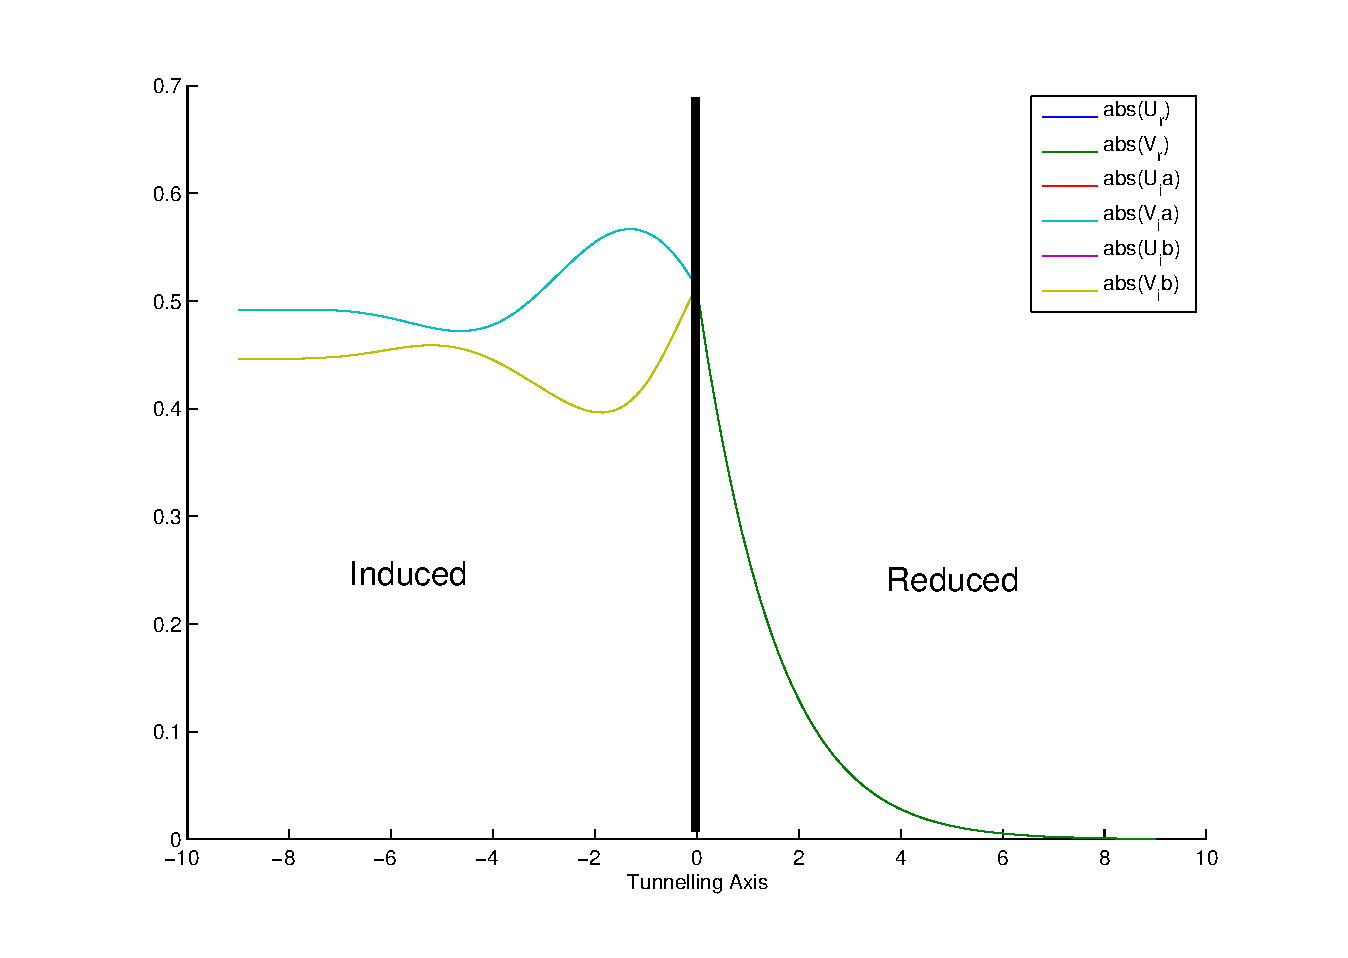
\includegraphics[width=10cm]{./Figures/3-2-2.eps}
		\rule{35em}{0.5pt}
	\caption[An Electron]{The shapes with $E=0.5$, subscript $r$ indicates reduced region while $i$ induced region. Notice that in reduced region, $u^*=v$.}
	\label{fig:Electron}
\end{figure}
 \begin{figure}[htbp]
\small
	\centering
		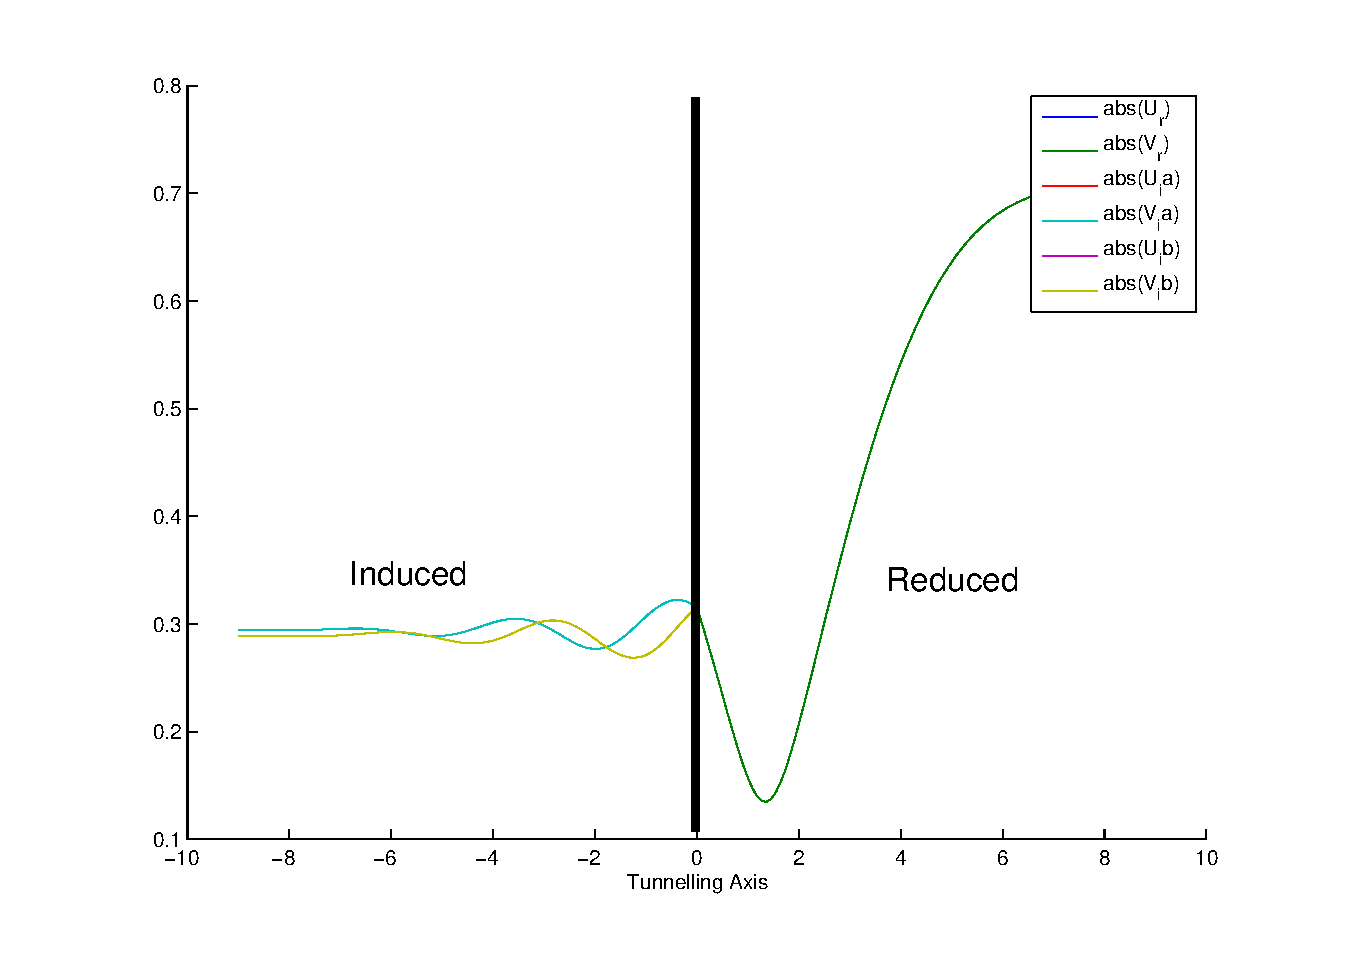
\includegraphics[width=10cm]{./Figures/3-2-3.eps}
		\rule{35em}{0.5pt}
	\caption[An Electron]{The shapes with $E=1$, subscript $r$ indicates reduced region while $i$ induced region}
	\label{fig:Electron}
\end{figure}

 \begin{figure}[htbp]
\small
	\centering
		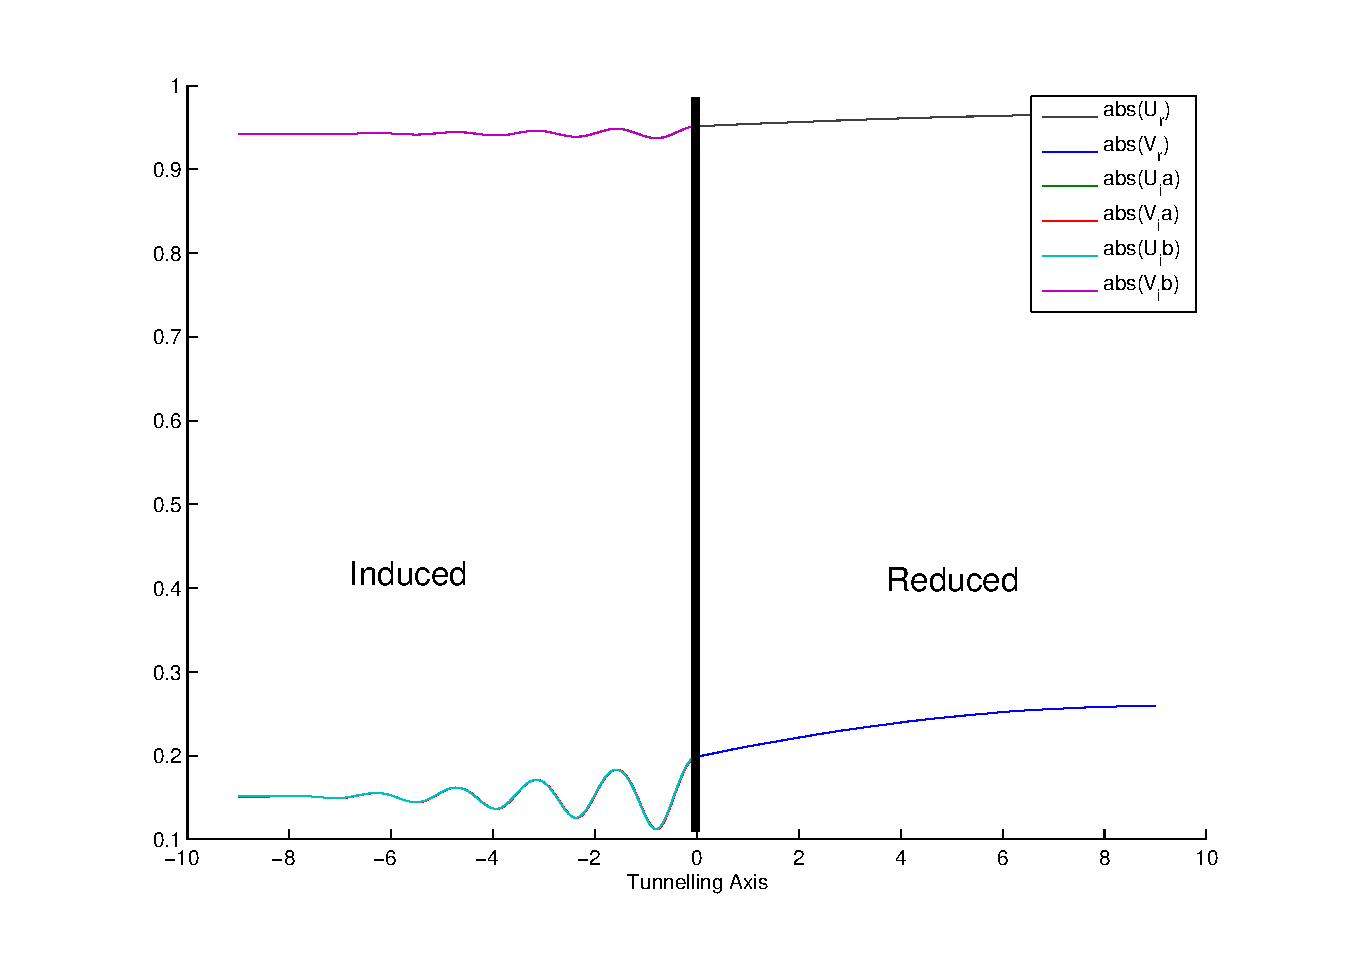
\includegraphics[width=10cm]{./Figures/3-2-4.eps}
		\rule{35em}{0.5pt}
	\caption[An Electron]{The shapes with $E=2$, subscript $r$ indicates reduced region while $i$ induced region}
	\label{fig:Electron}
\end{figure}

 \subsection{The Specific Case of BTK}
 First of all we check the reliability of our model. Ideally, BTK is a specific case of our discussion in this chapter; in other words, if we set $\Delta_R=1,\Delta_I=0$, we should see the results of BTK, Fig3.5.
Here are a set of figures, in which the deep blue one represents the BTK, the famous V-shape shown.
\begin{figure}[htbp]
\small
	\centering
		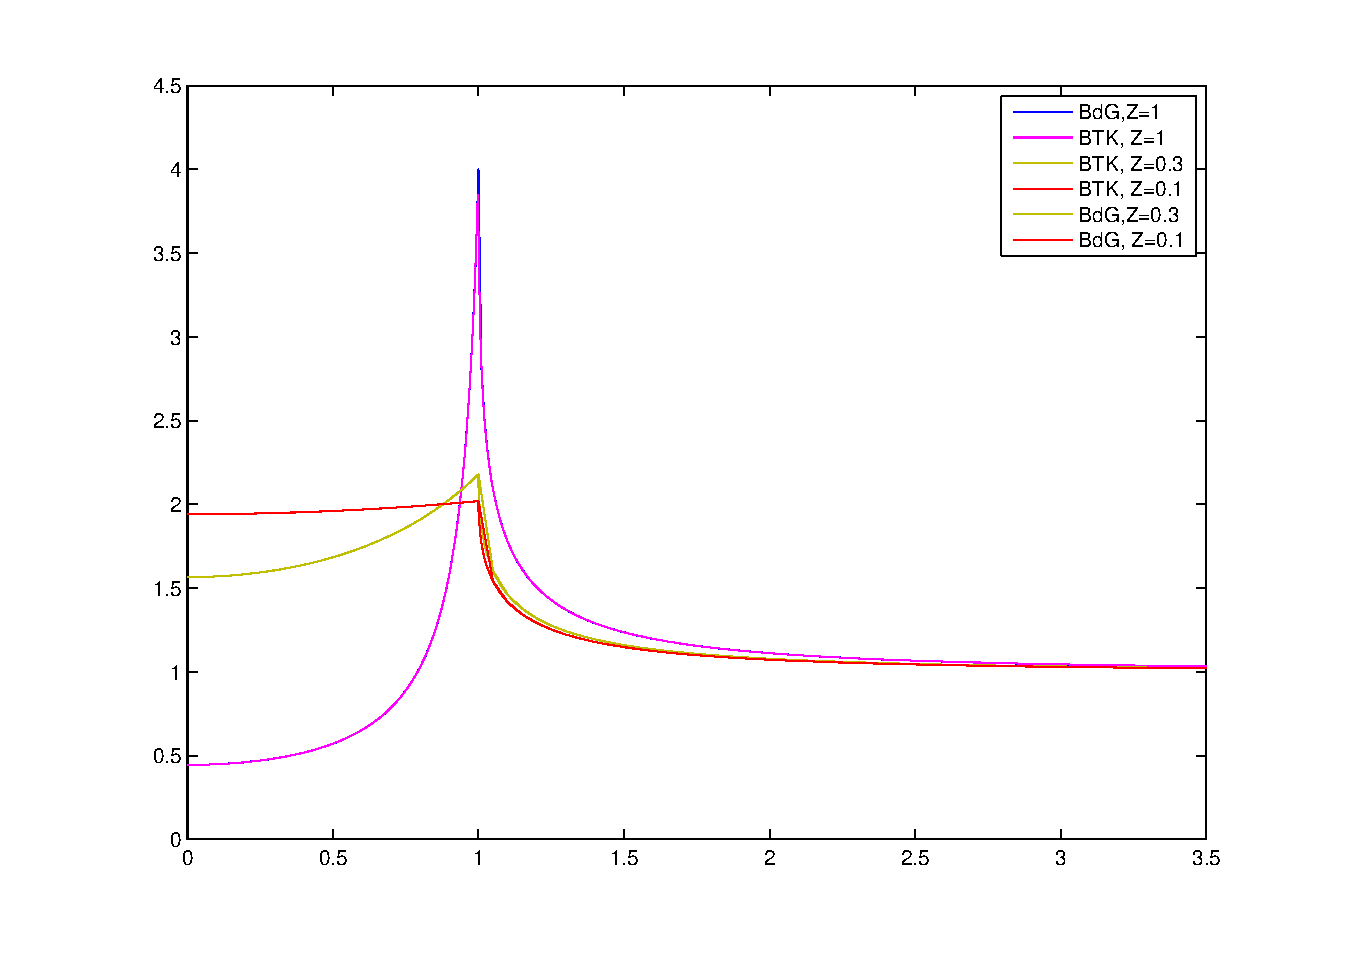
\includegraphics[width=10cm]{./Figures/3-2-8.eps}
		\rule{35em}{0.5pt}
	\caption[An Electron]{BTK case when we set $\Delta_R=1,\Delta_I=0$}
	\label{fig:Electron}
\end{figure}
 Also, when barrier hight $Z=0$, we should observe flat region with the value of $2$ in the middle, Fig.3.6.
\begin{figure}[htbp]
\small
	\centering
		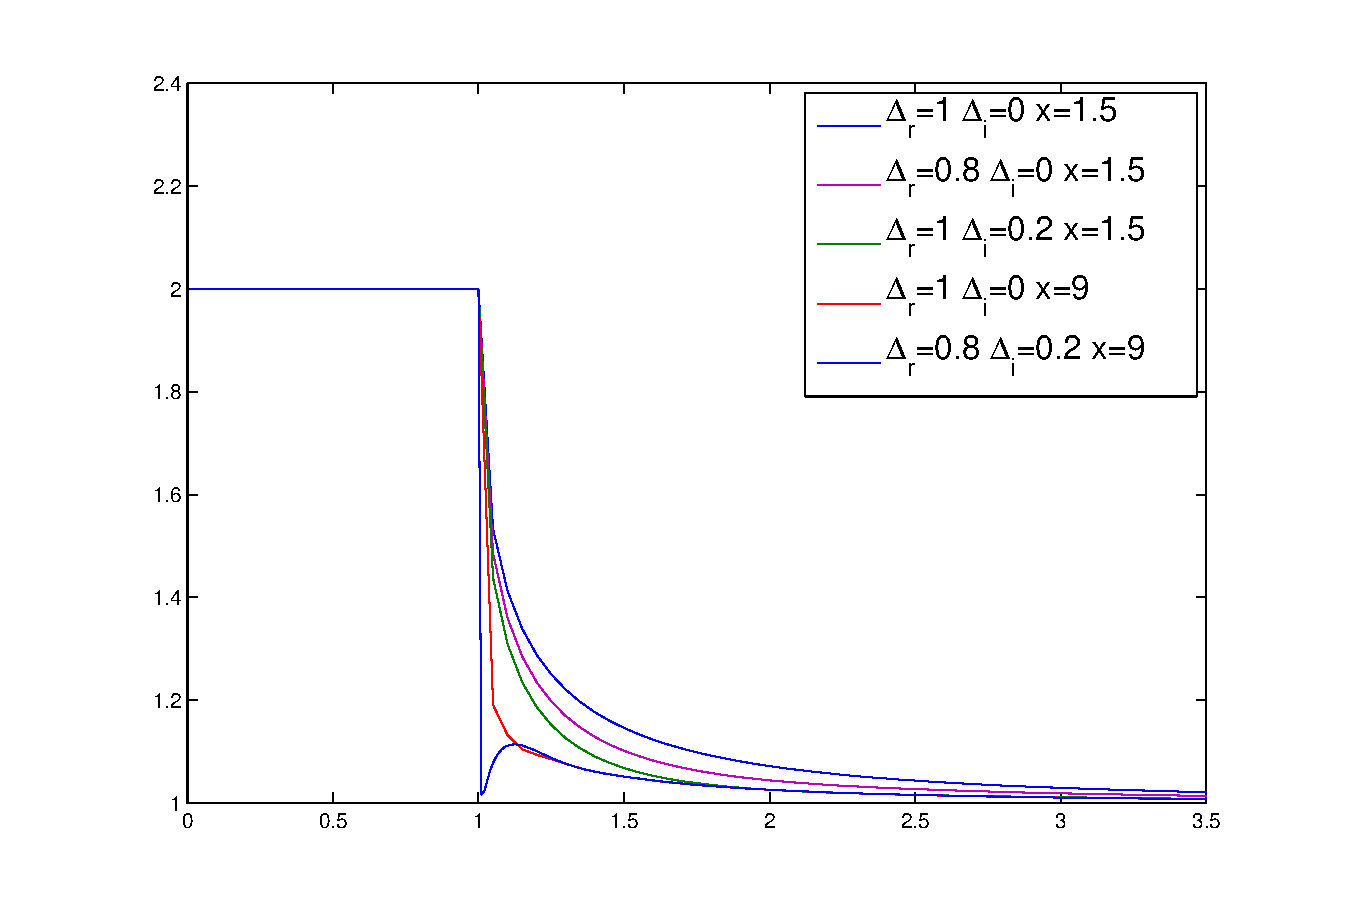
\includegraphics[width=10cm]{./Figures/3-2-9.eps}
		\rule{35em}{0.5pt}
	\caption[An Electron]{The flat region in the middle appears no matter what parameters we set}
	\label{fig:Electron}
\end{figure}

\section{Tunnelling Spectroscopy with Proximity Effect}
Similar to the procedure in the previous chapter, with solutions obtained, we first have a look at the kernel of the conductance.
\begin{eqnarray}
\sigma_T=1+A-B
\end{eqnarray}
\subsection{Proximity Effect with various parameters}
We draw a list of figures showing the change of the shape according to the varying reduced gap and induced gap, setting the coherence length as $\pi\xi_0=1$, Fig.3.7, Fig.3.8.
In addition, we plot another group of figures with $Z=0.3$, Fig.3.10-Fig.3.13.
\begin{figure}[htbp]
\small
\centering
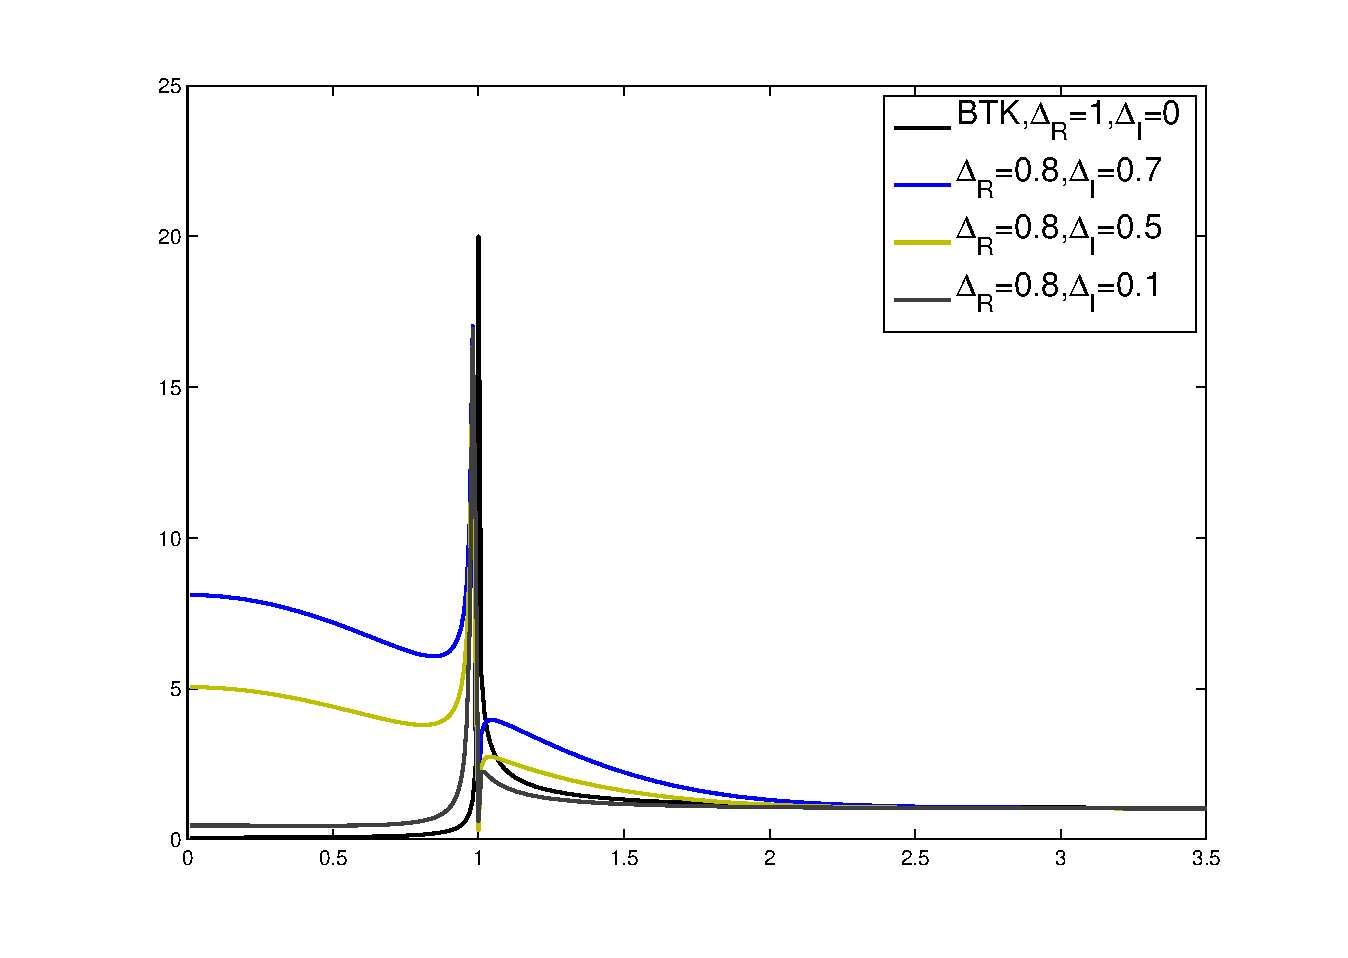
\includegraphics[width=10cm]{3-3-1.eps}
\caption{The figure indicates the difference with induced gap varying.$Z=3$.}
\label{fig:5}
\end{figure}
\begin{figure}[htbp]
\small
\centering
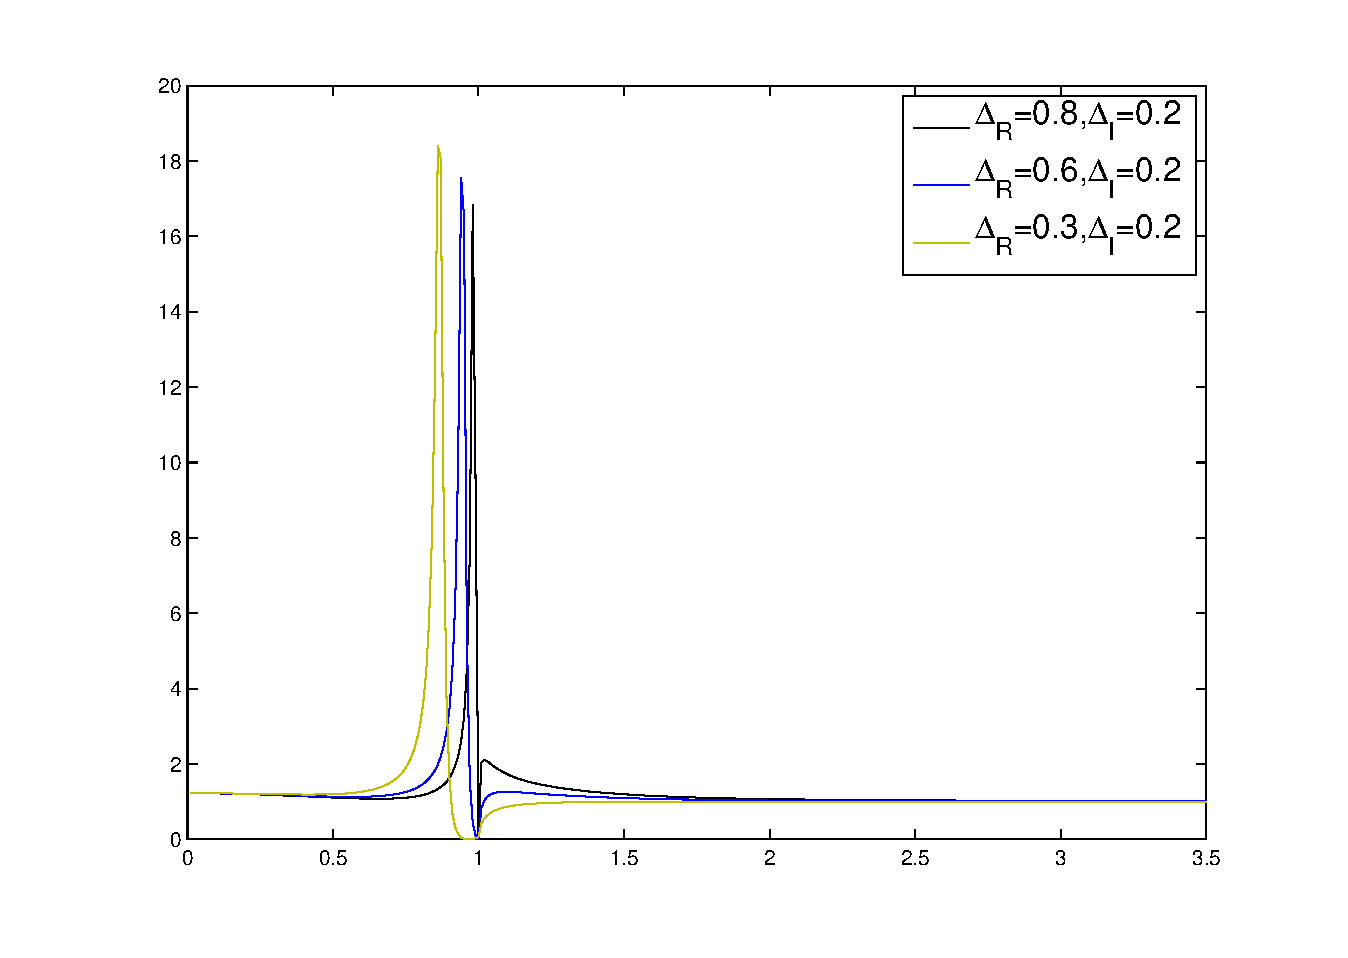
\includegraphics[width=10cm]{3-3-2.eps}
\caption{The figure indicates the difference with reduced gap varying.$Z=3$}
\label{fig:6}
\end{figure}

As a thought, the proximity domain certainly affects the behaviours of the transmission. Here I did research on the influences.
Fig.3.9 indicates the relationship between proximity domain and the shape of the conductance, with reduced gap 0.8 and induced gap 0.4.
\begin{figure}[htbp]
\small
\centering
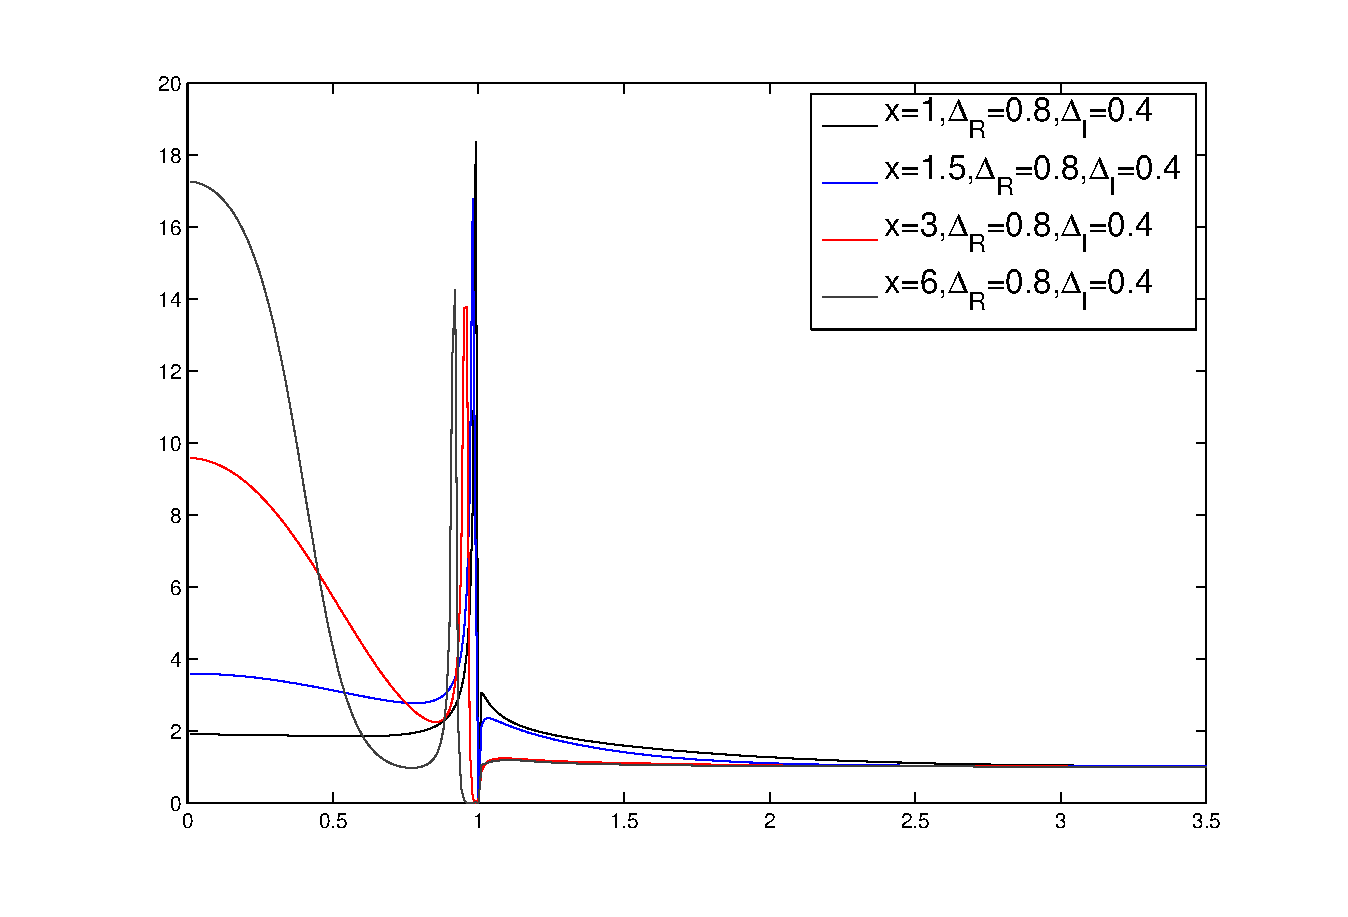
\includegraphics[width=10cm]{3-3-3.eps}
\caption{The proximity domains affects the left side of the shape significantly.$Z=3$}
\label{fig:7}
\end{figure}
\begin{figure}[htbp]
\small
\centering
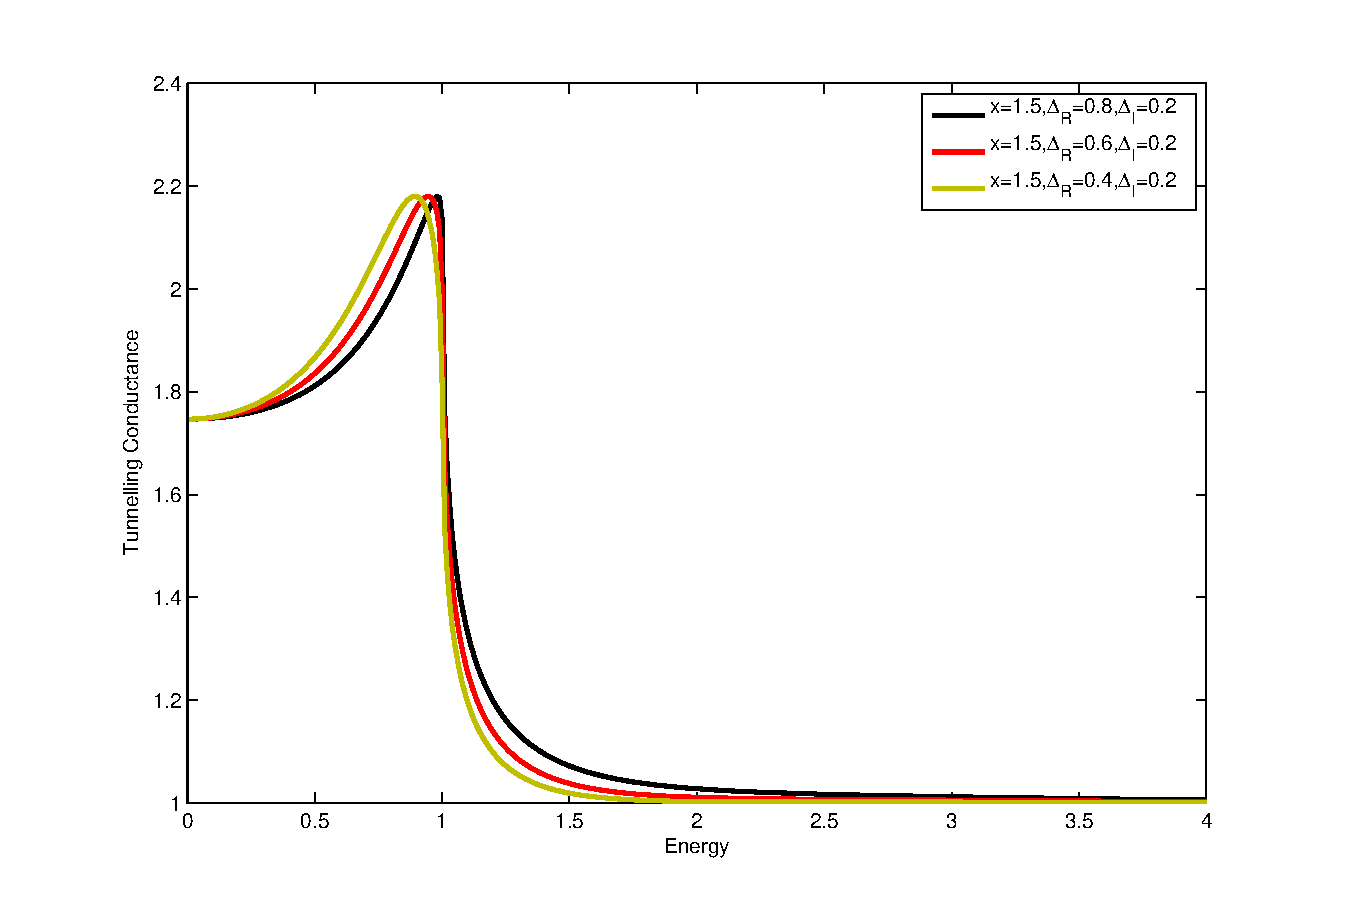
\includegraphics[width=10cm]{3-3-4.eps}
\caption{Low barrier hight.$Z=0.3$}
\label{fig:8}
\end{figure} 
\begin{figure}[htbp]
\small
\centering
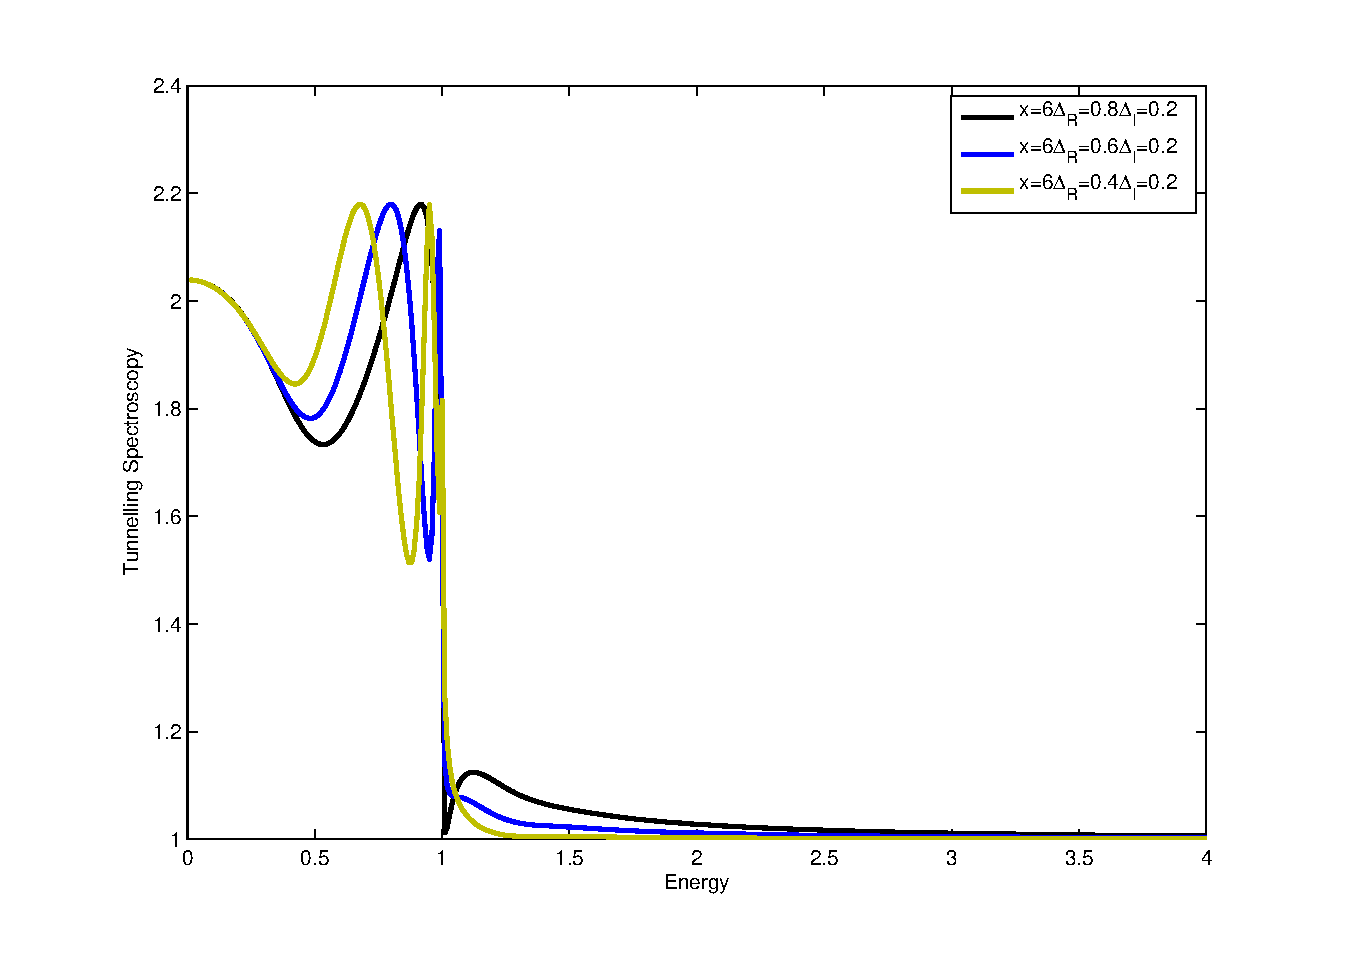
\includegraphics[width=10cm]{3-3-5.eps}
\caption{Some peaks show if thicker proximity domain is chosen at low barrier hight.$Z=0.3$}
\label{fig:9}
\end{figure}
\begin{figure}[htbp]
\small
\centering
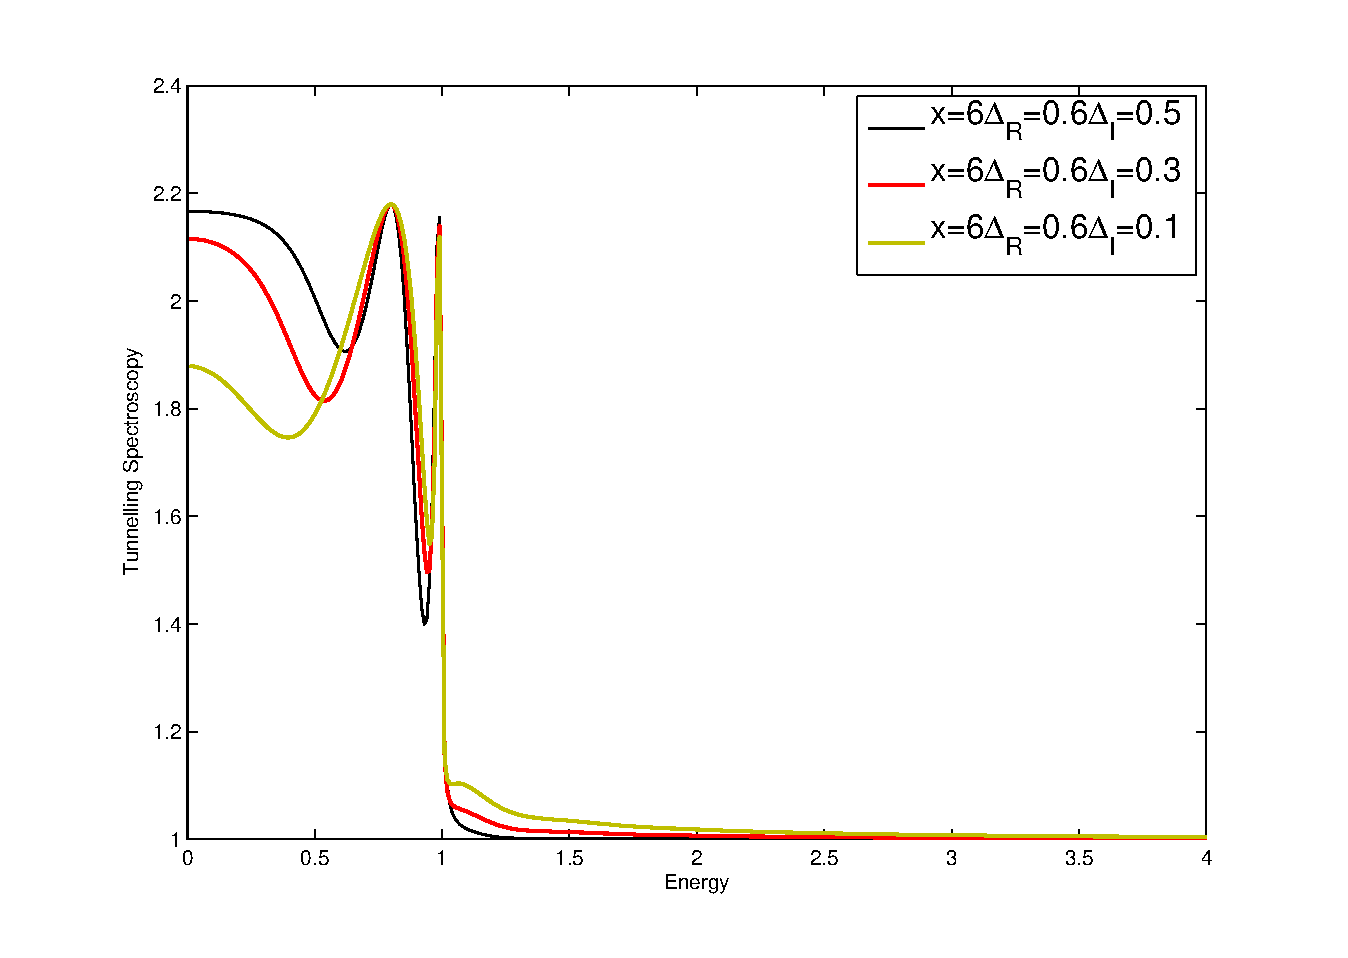
\includegraphics[width=10cm]{3-3-6.eps}
\caption{Some peaks show if thicker proximity domain is chosen at low barrier hight.$Z=0.3$}
\label{fig:10}
\end{figure}

We set the proximity effect parameters as $x_S=x_N=9,Z=0.3$, we obtain the Fig.3.16. Their physical meanings, however, remains to be discovered. In this figure, we obtained a number of peaks.
\begin{figure}[htbp]
\small
\centering
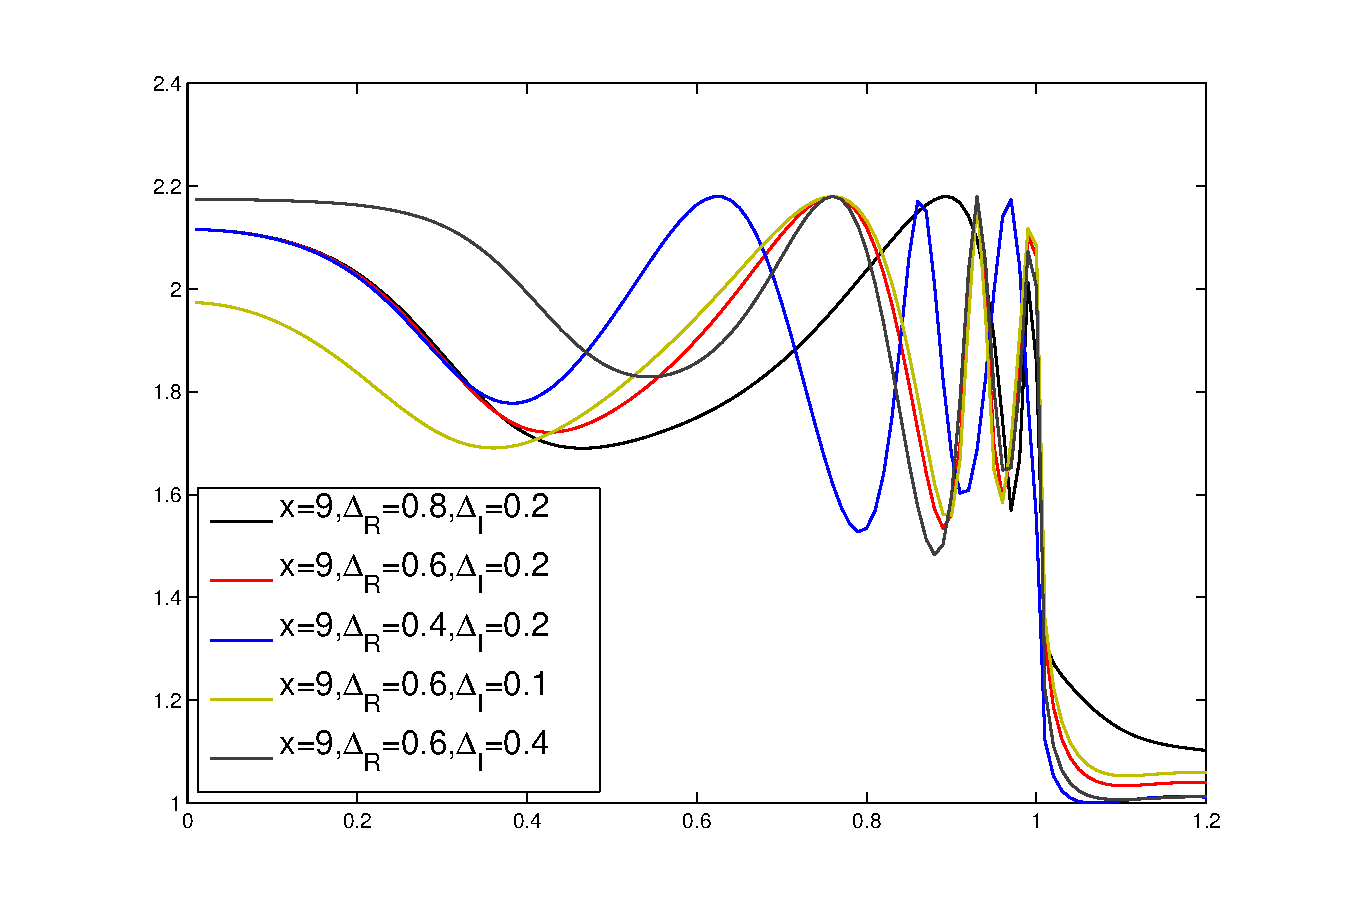
\includegraphics[width=10cm]{3-3-7.eps}
\caption{Some peaks show if thicker proximity domain is chosen at low barrier hight.$Z=0.3$}
\label{fig:10}
\end{figure}
\subsection{$s$ wave tunnelling spectroscopy with proximity effect}
The induced gap brings a bulk in the middle intead of the desired peaks and the function of reduced gap remains unknown. Here we make a small trial step moving to $s$ tunnelling spectroscopy, whose shapes though look like those of un-integrated ones.
In Fig.3.13, we could see the effects of induced gap. The induced gap creates a bulk in the middle.
\begin{eqnarray}
\sigma_T(E)=\DF{\int_0^{2\pi}d\varphi\int_{-\frac{\pi}{2}}^{\frac{\pi}{2}}d\theta \sigma_S(E)\cos\theta}{\int_{0}^{2\pi}d\varphi\int_{-\frac{\pi}{2}}^{\frac{\pi}{2}}d\theta\sigma_N\cos\theta}
\end{eqnarray}
\begin{figure}[htbp]
\small
\centering
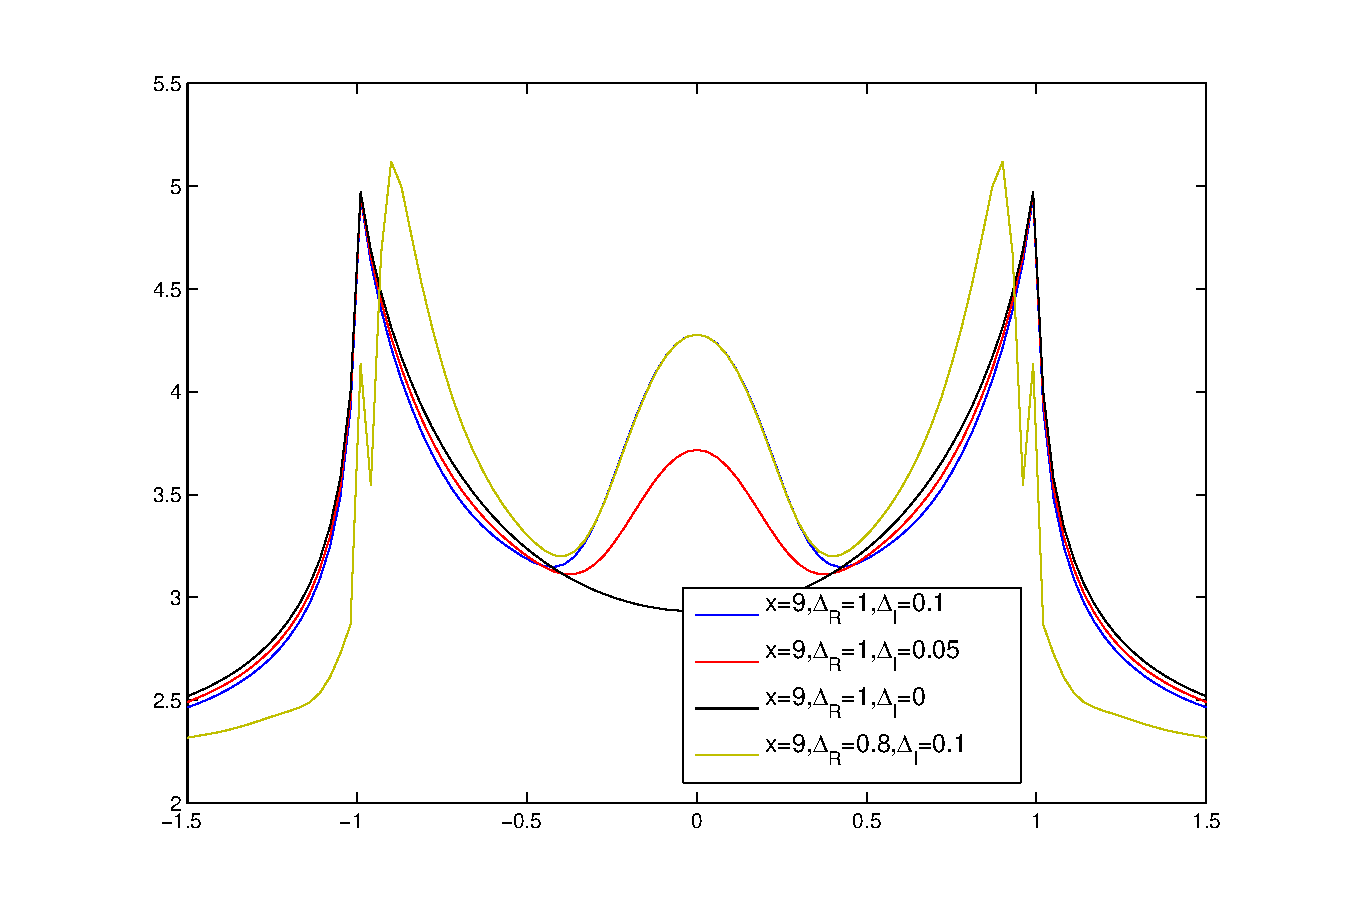
\includegraphics[width=10cm]{./Figures/3-3-8.eps}
\caption{The $s$-wave tunnelling spectroscopy. The induced gap creates a bulk in the middle of the figure}
\label{fig:10}
\end{figure}









